\chapter{绪\hskip 0.4cm 论}
\label{ch1}

\section{研究背景及意义}
信息物理融合系统(Cyber Physical System,CPS)\cite{wangzhongjie2011cpssurvey}是一种复杂的异构系统,主要具有以下两个特征:1)不确定性:该系统面向开放环境,受多种不确定因素影响,如天气突变、信号误差、人为失误等,因此在设计该系统时,我们要充分考虑多种不确定性的因素,以保障CPS 在不确定环境下的可信性;2)异构性:该系统除了包含计算机系统之外,还结合了机械、环境、土木、电子、生物、化学、航空等诸多工程领域的模型和方法,且各领域深度的融合,因此我们不仅仅需要设计和建模各个工程领域的模型,更要充分考虑各个领域之间的交互问题。因此,由于CPS的不确定性和异构性,使CPS的建模分析及验证面临巨大的挑战,已有的CPS研究已经针对CPS的建模、仿真做了大量的工作并相应的有了一些工具的支持,例如基于时间自动机理论的UPPAAL\cite{bulychev2012uppaal}可以很好的建模和验证系统的基于时间的行为,基于马尔科夫模型的Prism\cite{kwiatkowska2011prism}对概率系统的建模和验证提供了很好的支持,Modelica \cite{Fritzson1998Modelica}、Simulink\cite{zuliani2013bayesian} 等工具支持对连续的物理系统提供较好的建模仿真等等。然而,以上工作在解决CPS的建模仿真及验证问题上各有优势及不足。因此,想要更好的支持CPS系统各种性质的建模、仿真和验证,我们需要整合多种特定领域模型工具的建模、仿真及验证优势。为了解决这一问题,GEORG, H等人在论文\cite{Georg2014Analyzing}中提出了两种方法:一种是设计统一的建模仿真平台,该平台可以结合所有领域模型的优势并支持所有领域模型的建模仿真;另一种是使用协同仿真\cite{Bastian2011Master}技术,仍然是在各个领域模型的建模工具中进行建模,然后将各个领域建模工具建模出的模型根据统一标准转化为一种标准模型,最后根据这一标准提供的接口在仿真过程对模型进行仿真。Georg, H等人在文中也提到,第一种方案实现起来比较困难,所以建议使用第二种方案。经过协同仿真过程之后,我们可以得到不同领域模型融合在一起仿真的迹(trace),由于仿真迹的可读性不高,通过对仿真迹进行直接观察我们很难评估分析系统的行为。因此,LEGAY A等人提出了统计模型检测方法(Statistical Model Checking,SMC)\cite{Legay2010Statistical},该方法以模型的仿真迹和验证属性(Property)作为输入,最终将得到模型满足这一属性的概率值。统计模型检测方法提出以来,主要是用来对特定领域模型的行为进行定量的评估分析,在本文中我们用该方法来评估分析多个模型协同之后的行为。

本文提出了一种基于协同仿真及统计模型检测的信息物理融合系统定量评估分析方法,在该方法中我们使用协同仿真技术来对多个领域模型进行融合仿真并得到仿真的迹,然后对整个系统设计需要验证的属性,最后将仿真迹和验证属性输入到统计模型检测器中进行评估分析。对于该方法,我们主要需要解决两个问题,也是本文的两个重要的贡献点:(1)需要保证多个领域模型进行协同仿真时的正确性,即需要对多个模型进行协同时的协同行为进行验证;(2)由于统计模型检测需要消耗大量的仿真迹,且在协同仿真时产生仿真迹的过程尤为耗时,使得整个验证时间需要极大的时间开销,因此我们需要对统计模型检测算法进行改进,以更快的完成验证过程。解决了以上两个问题之后,我们本文提出的方法就可以很好的结合多种建模仿真的优势,并为准确高效的对CPS系统的建模、仿真和定量评估分析提供有效的支持。 


\section{国内外研究现状}

\subsection{信息物理融合系统}
信息物理融合系统的概念最早是由美国自然基金委提出,之后便获得了国内外的广泛关注。各个国家的科研人员从CPS的建模、验证分析等不同方面展开了深入的研究。CPS从2005年提出至今,它的发展得到了多国政府的大力资助和支持,并成为学术界、科技界研究的重点方向,具有很高的科学研究意义。同时,CPS也在工业界有了大量的案例应用,具有广阔的应用前景和商业价值。在美国,近些年举办了多次CPS的科研会议和研讨活动,针对CPS的理论、性能及安全性等问题展开了深入的探讨。美国科研人员的研究热点主要涉及嵌入式系统、网络信息安全等方面,并已经取得了较好的研究成果。例如:哥伦比亚大学伯克利分校设计的PTOLEMY平台对CPS系统的架构建模和仿真提供了工具支持。麻省理工学院 (Massachusetts Institute of Technology, MIT)设计了分布式智能机器人花园,提高了CPS各个节点之间的交互和实时通讯的效率。宾夕法尼亚工程学院了汽车导航软件GrooveNet,为车辆CPS系统的建模和仿真提供了一个良好的建模和仿真平台。Carnegie Mellon 大学将支持向量机预测模型和马尔科夫状态控制等方法应用于智能电网CPS系统的建模之中,来实现智能电网的调度控制。在欧洲,对于CPS的研究主要集中在理论研究方面。例如:在2008年,欧盟启动了 ARTEMIS (Advanced research and technology for embedded intelligence and systems) 项目, 将CPS作为一个重点的研究方向, 并创办了 “International Journal of Cyber-Physical Systems”专刊。法国自动化研究所设计的GEMOC平台对信息物理融合系统的建模提供了有效的支持。在中国,于2008年在北京召开了IEEE嵌入式研讨会, 将CPS作为接下来的重点研究方向。2010年, 国家863计划信息技术领域办公室和专家组在上海举办了 “CPS发展战略论坛”, 对CPS给以高度关注。武汉大学信息资源研究中心提出了结合云计算和下一代互联网的理念, 进行 CPS 语义中间件的设计, 研了究CPS 网络互联和自主交互等技术。华东师范大学使用形式化的方法对CPS进行了建模,并对其可信性进行了验证分析。此外, 清华大学、天津大学、同济大学等多所研究机构也对CPS进行了深入研究。

\subsection{协同仿真}
CPS包含信息和物理两个部分,并涉及各个领域。因此,对于CPS的各个属于不同领域的模块都有相应的工具及方法支持。对CPS的建模和仿真主要有两种方案: (1)开发一个统一的CPS建模平台,该平台支持CPS涉及的各个领域的建模和仿真 (2)将CPS的各个部分在不同的领域工具中建模,使用协同仿真技术在仿真阶段将不同领域模型融合在一起进行仿真。方法一到目前为止实现起来较为复杂,因此学术界对协同仿真技术进入了深入的研究。为了模拟CPS,H. Georg等人在论文\cite{Georg2014Analyzing}中提出整合CPS的不同仿真域来综合分析CPS中相互依赖的子系统。作为一种十分有效的CPS仿真技术,协同仿真可以将让CPS不同的领域模型在它们自己的专有仿真软件之中进行仿真并在特定的时间点进行模型之间的数据交互以到达模型的数据同步。功能模拟接口(Functional Mock-up Interface,FMI)\cite{Arnold2011FMI}是一个行业标准,它能够使用多个仿真引擎对复杂异构系统进行协同仿真,已被业界和学术界所采用。例如,J. Bastian等人在论文\cite{Bastian2011Master}中采用FMI标准和固定步长主算法来对异构系统进行协同仿真。实现了FMI标准的组件被称为功能模拟单元(Functional Mock-up Unit,FMU)\cite{Tripakis15}, D.Broman等人在论文\cite{Broman2013Determinate}中讨论了在协同仿真过程中,异构系统中各个FMU进行组合时的确定性问题。此外,他们对FMI标准进行了扩展并提出了支持回滚和步长预测主算法,以提高协同仿真的准确度和效率。在论文\cite{Cremona2016FIDE}中,F. Cremona等人介绍了基于FMI标准构建的协同仿真集成开发环境FIDE。在我们之前的研究工作\cite{LiuJWCD16}中,我们基于FMI标准实现了prism和modelica模型的协同仿真,并且提出了一种基于事件的协同仿真算法,一定程度上提高了协同仿真的效率。由于协同仿真存在不确定性,因此在进行仿真之前我们应该保证整个系统的协同行为的正确性。针对协同行为正确性的验证,相关研究人员也做了一定的研究工作。例如:P.G. Larsen等人在论文\cite{Larsen2016Integrated}中使用形式化规约语言CSP对FMI的语义进行了形式化的描述,并使用验证工具FDR3对得到的模型进行了形式化的验证分析。

\subsection{分布式技术}
分布式技术与传统的集中式的处理技术相对应,它是一种基于网络的多个计算机并行计算的处理技术。随着信息技术的发展,系统变得愈加复杂,因此对计算机的处理能力有了更高的要求。在一定程度上,单台计算机的处理能力已经很难满足当前复杂系统的计算需要。分布式技术使用多台低成本的计算机达到了十分高的计算性能。该技术近些年来发展十分迅速,并且在大数据存储、高复杂度的数据计算等方面发挥了重要作用。当前分布式技术引起了学术和工业界的高度重视,并且已经在科研、医疗、教育等方面有了许多应用案例。例如:SETI@home通过使用参与分布式的计算集群来对射电望远镜收到的海量信号进行计算分析,以确定还有无类似地球生物的生命存在,寻找宇宙生命体。Climateprediction工程是一个分布式计算技术在气象预测领域的一个成功案例,该项目将收集到的海量气象数据发放给多台计算机,每台计算机都会对接收到的数据继续计算并把计算结果返回,最终组建了地球的气象模型。Folding@home是分布式计算技术在医疗领域的一个成功的应用案例,这个项目基于多个计算机组成的超高计算性能来研究蛋白质折叠、聚合及由此引起的疾病。

\subsection{统计模型检测}
统计模型检测概念 基本算法
在论文\cite{Grosu2005Monte}中,R.Grosu等人首次提出了统计模型检测的概念。统计模型检测基于仿真和统计技术,来验证某个模型满足某一验证属性的概率或者是验证某个模型满足某一属性的概率是否大于或小于某个特定的阈值。根据最终验证目标的不同,可以将统计模型检测算法分为定性和定量算法。定性算法回答了“系统满足属性的概率是否大于或等于某个特定阈值”的问题,最终得到的结果是一个布尔值。当前经典的定性统计模型检测算法主要有Single Sampling Plan(SSP)\cite{sen2004statistical}算法、Sequential Probability Ratio Test(SPRT)\cite{wald1945sequential}和Bayesian Hypothesis Testing(BHT)\cite{zuliani2013bayesian}算法。SSP算法最早被Sen等人提出,但是该算法难以确定算法收敛需要的样本数量和接受假设的阈值,Younes等人在论文\cite{younes2005verification}中提出使用二叉搜索的算法来近似得到这两个参数值。在之后,Younes等人在论文\cite{younes2005verification,younes2006statistical}中还提出了SPRT算法的设计和算法实现,用来提高定性统计模型检测算法的效率。Zuliani等人也基于贝叶斯统计理论提出了BHT算法来提高定性统计模型检测算法的效率。定量算法用来直接得到模型满足某一验证属性的概率,当前经典的定量统计模型检测算法主要有Approximate Probabilistic Model Checking(APMC)\cite{herault2004approximate}算法和Bayesian Interval Estimation(BIE)\cite{jha2009bayesian}算法,APMC算法用满足属性的样本数量除以所有得到的样本数量来得到满足验证属性的概率,并用Chernoff-Hoeffding界来限定误差。Clarke等人基于贝叶斯统计理论提出了BIE算法以提高定量统计模型检测的效率。Kim等人在论文\cite{Kim2012Statistical}给中出了以上算法的对比分析,实验结果表明以上几种算法均可以对模型进行有效的定量或定性的评估分析。 对于定性统计模型检测算法,SPRT和BHT算法比SSP算法更加高效,且当概率阈值远离最终的真实概率时,BHT比SPRT高效,否则BHT的效率明显低于SPRT。 对于定量的统计模型检测算法,Zuliani等人在论文\cite{zuliani2013bayesian}中对比了它们使用的样本数量并得出结论,BIE算法比APMC算法更加高效。

由于统计模型检测算法需要消耗大量的仿真样本,其验证过程较为耗时,因此其效率问题受到了广泛的关注。相关研究人员提出了使用抽象和学习的方法来提高统计模型检测的效率。例如:在论文\cite{Kumar2014Efficient}中,Kumar等人通过预测可能的结果或事件的发生来学习预测模型并进行验证,这种方法可以直接应用现有的机器学习技术,但很难得到精确的误差评估。在论文\cite{Basu2012Statistical}中,等人使用在概率等价的基础上,使用抽象的方法将原始的模型进行简化,然后对简化之后的模型进行验证,该方法在保证准确度的基础上一定程度提高了统计模型检测的效率。在我们之前的工作\cite{jiangkaiqiang2016}中,我们使用抽象和学习的方法将原始模型划分成了多个子模型,然后对多个子模型进行验证分析,最终将验证结果合并。该方法可以有效提高统计模型检测的效率并将误差控制在了一定的范围之内。在论文\cite{younes2005ymer}中,Younes等人指出统计模型检测算法可以进行分布式设计,并且他们还提出了一种方法来消除分布式设计中可能出现的偏差。接下来,Peter Bulychev等人在论文\cite{Bulychev2012Checking}中对BHT算法给出了分布式的设计和实现。

当前,已经有越来越多的工具支持了统计模型检测算法。Ymer\cite{younes2005ymer}和Vesta\cite{sen2005vesta}最早对统计模型检测算法提供了支持。Vesta采用了SSP算法的一个变种,而Ymer采用的是SPRT算法,且Ymer工具的效率要高于Vesta。目前对SMC算法提供较好支持的工具是UPPAAL-SMC和Prism,UPPAAL-SMC和Prism都实现了定性的SPRT算法和定性的BIE算法,同时它们还实现了都实现了Confidence Interval(CI)\cite{brown2001interval}算法。UPPAAL-SMC时间自动机理论,对时间和连续性有较好的支持且有图形化的建模界面;Prism基于马尔科夫模型,对随机性和不确定性有较好的支持,且使用Reactive Modules Language(RML)建模。Plasma Lab\cite{boyer2013plasma}是一个统计模型检测算法的集成工具,其中实现了BHT,BIE,SPRT等多种统计模型检测算法。用户可以根据需要选择要用的统计模型检测算法并输入参数进行模型的评估分析,该工具同样使用RML进行建模。


\section{本文技术路线及主要研究内容}
信息物理融合系统是异构系统,本文针对这种异构系统的验证提出了一种解决方案,图\ref{pa-fra}为本文的技术路线图,本文的技术路线大致如下:

(1)我们通过对该系统进行分析,提取出该系统的信息部分(Cyber part)和物理部分(Physical part),除此之外我们根据自己需要验证的行为属性定义约束(Constraint)。

(2)使用系统建模语言((Systems Modeling Language,SysML)\cite{Dori16} 建模语言对提取出的信息部分和物理部分进行建模,将信息系统和物理系统的组件使用SysML的块定义图(SysML Block Definition Diagram,BDD)图进行建模,同时使用SysML的内部框图(SysML Internal Block Diagram,IBD)图来描述系统中各个组件之间的关联。

(3)SysML只是用来建模组件内部结构和组件之间的关联,该模型不可直接进行仿真运行,因此我们将SysML BDD图建模的模型使用FMU进行实现,同时将SysML IBD图描述的系统组件关系转化为FMU之间相互依赖的接口配置文件,此时,我们只需要再设计好协同仿真的主算法(Master Algorithm)就可以进行异构系统的协同仿真。然而,在进行协同仿真之前,我们首先要保证各个FMU之间的协同是正确的,要确保FMU之间协同行为的正确性,我们需要验证主算法的正确性及各个FMU之间的连接顺序及数据交换的正确性。在本文中,我们基于时间自动机设计了一个协同行为正确性验证的验证器,我们将系统的多个FMU、协同仿真的主算法以及FMU之间的接口配置文件输入到该协同行为的验证器之中即可验证当前系统协同行为的正确性,如果验证通过则说明我们当前的模型即为正确的模型,如果验证不通过,则需要修改当前系统的协同行为,直到得到验证通过的模型之后再输入到仿真器中进行仿真。

(4)我们在进行系统的验证分析时,首先需要验证的系统模型,同时我们还需要验证的属性(Property),我们将(1)中得到的约束进行形式化描述,即可得到验证属性(该验证属性根据约束的不同可以是BLTL/ALTL/GSCL等等,本文主要使用了BLTL作为验证属性)。

(5)将通过第三步验证的模型(Verified Model)及第四步得到的验证属性输入到异构系统验证器(co-verification)之中进行验证分析,首先将模型输入到仿真器(Simulator)之中进行仿真或协同仿真(Co-simulation)并得到仿真迹(Traces),然后将得到的仿真迹和验证属性输入到模型验证器(Checker)之中来验证该迹是否满足某条特定的验证属性,得到结果满足为1,不满足为0,我们将该验证是否满足的结果称为观察值(Observations),多条仿真迹对于一条特定的验证属性会得到多个观察值。最后将得到的观察值输入到统计分析算法中进行统计分析,并得到评估结果。
\begin{figure}[htbp]
	\centering
	{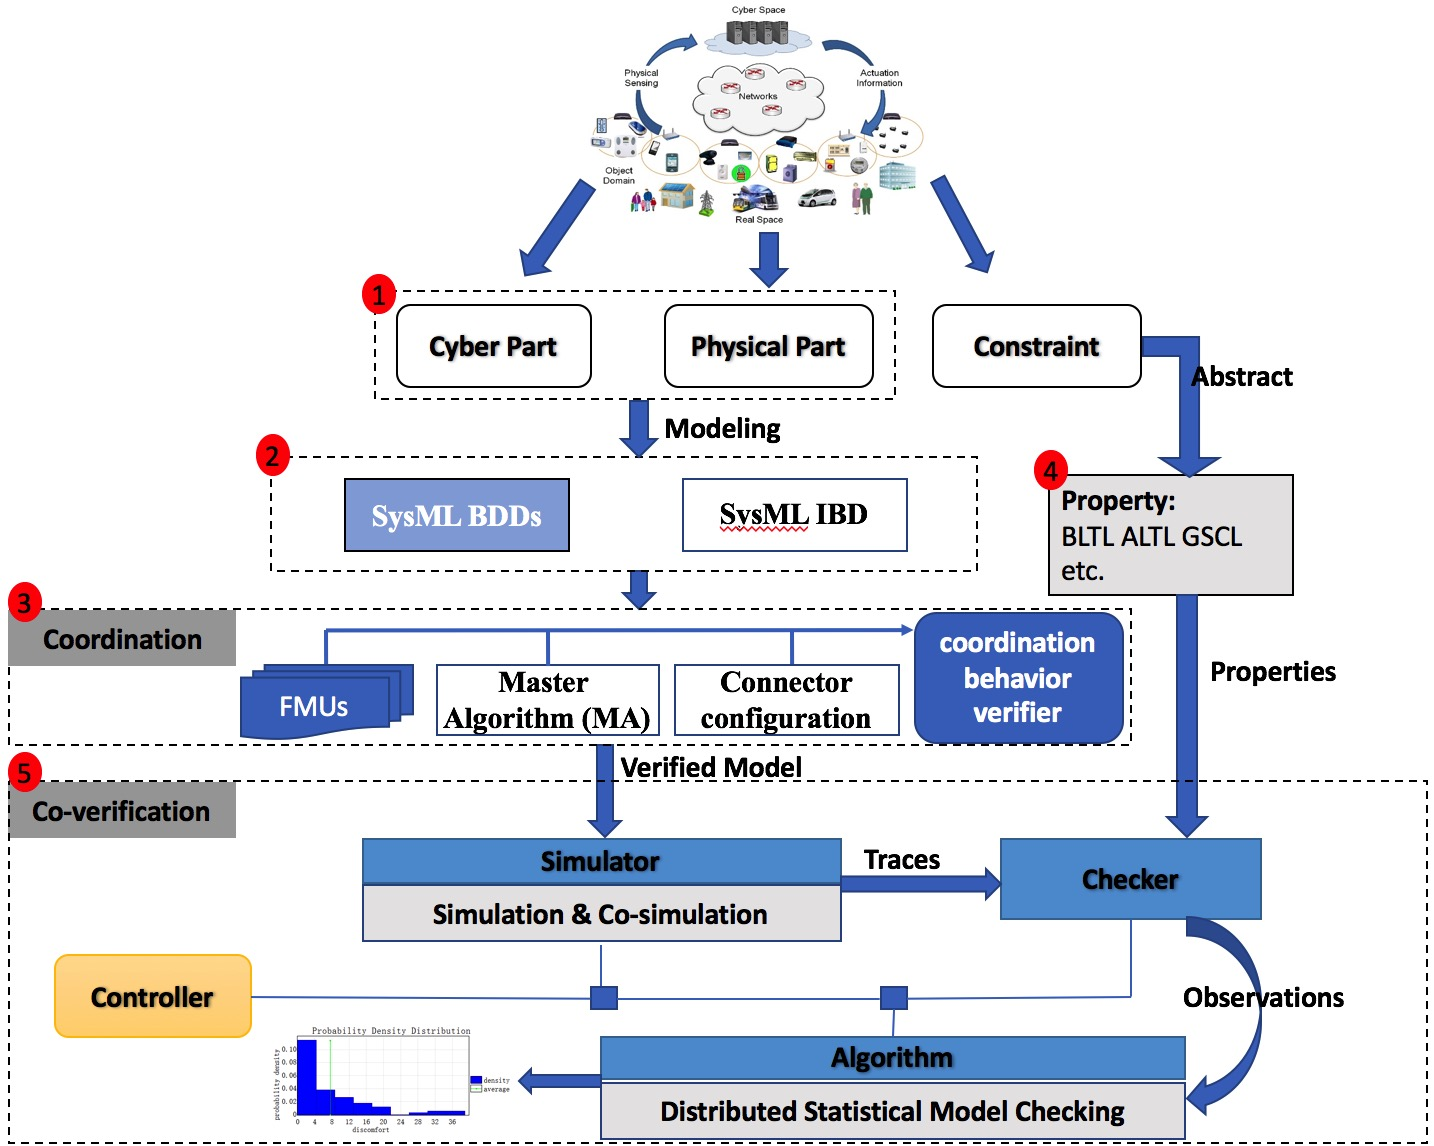
\includegraphics[width=5.0in]{fig/1/paper-framework.jpg}}
	%\vspace{0.10in}
	\caption{论文技术路线图}\label{pa-fra}
\end{figure}

\textbf{本文的具体研究内容和贡献点总结如下}:
\begin{enumerate}
	\item 使用SysML建模语言建模整个系统的架构,使用SysML的BDD图建模系统组件,使用SysML的IBD图来描述系统中各个组件的关联关系。
	\item 基于FMI标准实现SysML描述的系统模型,将SysML的BDD图建模的系统组件包装成FMU,并将各个组件的关联关系转化为FMU之间的接口配置文件。
    \item 使用时间自动机理论验证了基于FMI标准的多个FMU的协同行为,使用时间自动机将协同仿真的主算法进行形式化描述,并使用UPPAAL模型检测器来验证主算法的正确性;提出了一种从FMU到时间自动机的映射标准,通过此标准用时间自动机将多个FMU进行编码,并用时间自动机之间的通道(channel)来描述多个FMU之间的关联关系,最终将多个FMU及FMU之间的关联关系使用一个时间自动机网络进行了形式化描述,将该时间自动机网络输入到UPPAAL之中进行验证从而来验证协同行为的正确性。
    \item 提出了一种基于抽象和学习的分布式统计模型检测算法,在将误差控制在有效范围之内的基础上大大提高了统计模型检测的效率。
\end{enumerate}

\section{本文组织结构}
本文共分七章,组织结构如下:

第一章介绍了本文的研究背景及意义,并从四个方面阐述了该研究领域的国内外研究现状,其中包括信息物理融合系统的形式化建模、分布式技术、协同仿真及统计模型检测的研究现状。之后,给出了本文的技术路线和主要贡献点。最后,总结了论文组织结构。

第二章介绍了相关预备知识。首先给出了FMI标准的主要概念及定义,之后给出了概率有界线性时态逻辑、时间自动机及FMU的语法和语义定义。

第三章介绍了基于时间自动机理论来验证异构系统协同行为正确性的方法,首先我们给出了该方法的技术框架,之后我们详细描述了如何用时间自动机理论来验证协同仿真的主算法,以及如何验证整个异构系统的协同行为的正确性。

第四章重点阐述了如何用统计模型检测算法来对异构系统进行验证分析,也是本文的主要内容。首先,介绍了如何基于FMI标准对异构协同进行协同仿真并得到仿真迹,然后提出了一种基于抽象和学习的统计模型检测算法来提高统计模型检测的效率。最终,我们将协同仿真和该高效的统计模型检测算法进行结合,以此来对异构系统进行验证分析。

第五章主要介绍工具及程序实现。首先简单介绍了我们设计的异构系统验证工具(Co-SMC工具)。之后,给出了Co-SMC工具的详细设计及程序实现。

第六章给出了两个案例,通过使用本文提出的方法对这两个案例进行建模、仿真和分析来验证本文提出方法的有效性。

第七章为总结和展望,总结了本文提出的基于协同仿真和统计模型检测的信息物理融合系统验证方法,并讨论了其优点和不足,指出了未来要进一步进行研究的工作。
\section{本章小结}
本章首先说明了选题的背景和意义,指出了由于CPS的异构性而导致CPS系统的验证分析面临巨大挑战;接着介绍了信息物理融合系统、分布式技术、协同仿真及统计模型检测的研究现状;最后给出了本文的技术路线、主要贡献点和组织结构。下一章将介绍本文涉及到的预备知识及概念。
